\section{Week 11 - 04.05.2026 - The Inverse Laplace Transform and Application to Differential Equations}

\begin{recall}[Recall from last time:]
\begin{theorem}[Lerch's Theorem for Inverse Laplace Transform]
Suppose that $f:[0,+\infty)\rightarrow \C$ is a piecewise continuous function and for some $\gamma \in \R$, $F(z) = \Lap[f](z)$ is holomorphic on the region $\{z : \Re(z) \ge \gamma\}$ and the limit
$$\lim_{T\rightarrow+\infty} \int_{-T}^{T} F(\gamma+is) \cdot e^{(\gamma+is)t} \dd s$$
exists for all $t \ge 0$. (Both conditions are automatically true if some $\gamma_{c} < \gamma$ is an abscissa of convergence for $f$). Then:
\begin{align*}
f(t) &= \frac{1}{2\pi} \int_{-\infty}^{+\infty} F(\gamma+is) \cdot e^{(\gamma+is)t} \dd s \\
&= \frac{1}{2\pi i} \int_{\gamma-i\infty}^{\gamma+i\infty} F(z) \cdot e^{zt} \dd z
\end{align*}
\end{theorem}
\end{recall}

\begin{center}
\begin{tikzpicture}[scale=1.5]
    % Fill right half plane
    \fill[yellow!30] (1, -2) rectangle (4, 2);
    
    % Axes
    \draw[thick, ->] (-1, 0) -- (4, 0) node[right, scale=1.2] {$\Re$};
    \draw[thick, ->] (0, -2) -- (0, 2) node[above, scale=1.2] {$\Im$};
    
    % Abscissa of convergence
    \draw[dashed, red] (1, -2) -- (1, 2) node[below right] {$\Re(z) = \gamma_c$};
    
    % Integration line
    \draw[thick, teal, decoration={markings, mark=at position 0.5 with {\arrow{>}}}, postaction={decorate}] (2, -1.5) -- (2, 1.5);
    \draw[thick, teal, decoration={markings, mark=at position 0.2 with {\arrow{>}}}, postaction={decorate}] (2, -1.5) -- (2, 1.5);
    \draw[thick, teal, decoration={markings, mark=at position 0.8 with {\arrow{>}}}, postaction={decorate}] (2, -1.5) -- (2, 1.5);
    \node[teal] at (2, -1.5) [below right] {$\Re(z) = \gamma$};
\end{tikzpicture}
\end{center}

\textbf{Note:} The above integral might not converge absolutely (e.g., if $f(t)=1$ for $t \ge 0$, $F(z) = \frac{1}{z}$). So we just mean the principal value:
$$\frac{1}{2\pi} \cdot \lim_{T\rightarrow+\infty} \int_{-T}^{+T} F(\gamma+is) e^{(\gamma+is)t} \dd s.$$

\begin{remark}[Remarks]
\begin{enumerate}
    \item $f$ is uniquely determined by $\Lap[f]$ by this formula (Lerch's theorem).
    \item The condition on the existence of the limit $\lim_{T\rightarrow+\infty} \int_{-T}^{T} F(\gamma+is) \cdot e^{(\gamma+is)t} \dd s$ is automatically true if:
    $$\int_{-\infty}^{+\infty} |F(\gamma+is)| \dd s < +\infty.$$
\end{enumerate}
\end{remark}

\subsection{Example of Inverse Laplace Transform}

\begin{example}
Let $F(z) = \frac{1}{(z+1)(z+2)^2}$. Find $f : [0, +\infty) \rightarrow \R$ such that $\Lap[f] = F$.

There are two ways to do it:

\textbf{Method 1: Partial Fractions}
Note that
$$\frac{1}{(z+1)(z+2)^2} = \frac{1}{z+1} - \frac{1}{z+2} - \frac{1}{(z+2)^2}$$
Since we know that $\Lap[e^{-t}] = \frac{1}{z+1}$, $\Lap[e^{-2t}] = \frac{1}{z+2}$, and $\Lap[t e^{-2t}] = \frac{1}{(z+2)^2}$, we find:
$$f(t) = e^{-t} - e^{-2t} - t e^{-2t}$$
(By uniqueness of Laplace transforms, that's enough. Usually, this is the fastest way.)

\textbf{Method 2: Contour Integration (Inverse Laplace transform combined with the Residue Theorem)}
Using the formula for the inverse Laplace transform:
$$f(t) = \frac{1}{2\pi} \int_{-\infty}^{+\infty} F(\gamma+is) e^{(\gamma+is)t} \dd s$$
Let $h(z) = F(z) \cdot e^{zt} = \frac{e^{zt}}{(z+1)(z+2)^2}$.
Poles for $h$: $z = -1, -2$.
So we can choose $\gamma = 0$: $F$ is holomorphic on $\{z : \Re(z) > -1\}$ which contains $\{\Re(z) \ge 0\}$.
Also, $\int_{-\infty}^{+\infty} |F(\gamma+is)| \dd s < +\infty$.
\end{example}

Inverse Laplace transform:
$$f(t) = \frac{1}{2\pi} \int_{-\infty}^{+\infty} h(\gamma+is) \dd s = \frac{1}{2\pi i} \int_{-i\infty}^{+i\infty} h(z) \dd z$$

\begin{center}
\begin{tikzpicture}[scale=1.5]
    % Axes
    \draw[thick, ->] (-2.5, 0) -- (1.5, 0) node[right, scale=1.2] {$\Re$};
    \draw[thick, ->] (0, -2.5) -- (0, 2.5) node[above, scale=1.2] {$\Im$};
    
    % Curves
    \draw[thick, red, decoration={markings, mark=at position 0.3 with {\arrow{>}}, mark=at position 0.8 with {\arrow{>}}}, postaction={decorate}] (0, -2) arc (-90:-270:2);
    \draw[thick, red, decoration={markings, mark=at position 0.3 with {\arrow{>}}, mark=at position 0.8 with {\arrow{>}}}, postaction={decorate}] (0, -2) -- (0, 2);
    
    % Labels
    \node[red] at (0, 2) [right] {$+ri$};
    \node[red] at (0, -2) [right] {$-ri$};
    \fill[red] (0, 2) circle (1.5pt);
    \fill[red] (0, -2) circle (1.5pt);
    
    \node[blue, scale=1.2] at (-1.5, 1) {$C_r$};
    \node[blue, scale=1.2] at (0.3, 0.5) {$L_r$};
    
    % Poles
    \fill[black] (-1, 0) circle (1.5pt) node[below right] {$-1$};
    \fill[black] (-2, 0) circle (1.5pt) node[below left] {$-2$};
\end{tikzpicture}
\end{center}

Define the curves: 
$L_r : [-r, r] \rightarrow \C, s \mapsto is$
$C_r : [\frac{\pi}{2}, \frac{3\pi}{2}] \rightarrow \C, \theta \mapsto r \cdot e^{i\theta}$
$\Gamma = L_r \cup C_r$ (closed loop, counter-clockwise oriented).

When $r > 2$, $\Gamma$ encloses all the poles of $h$ (namely $z=-1, -2$). Applying the residue theorem:
$$\int_{\Gamma} h(z) \dd z = 2\pi i \left( \Res_{z=-1}(h) + \Res_{z=-2}(h) \right).$$

Since $h(z) = \frac{e^{zt}}{(z+1)(z+2)^2}$:
\begin{itemize}
    \item \textbf{At $z=-1$ (Simple pole):}
    $$\Res_{z=-1}(h) = \lim_{z\rightarrow-1} ((z+1)h(z)) = \lim_{z\rightarrow-1} \left( \frac{e^{zt}}{(z+2)^2} \right) = e^{-t}$$
    \item \textbf{At $z=-2$ (Pole of order 2):}
    \begin{align*}
    \Res_{z=-2}(h) &= \lim_{z\rightarrow-2} \left( \frac{\dd}{\dd z} \left( (z+2)^2 h(z) \right) \right) \\
    &= \lim_{z\rightarrow-2} \left( \frac{\dd}{\dd z} \left( \frac{e^{zt}}{z+1} \right) \right)
    \end{align*}
\end{itemize}

\begin{verification}[Correction of the derivative limit at $z=-2$]
Let's rigorously evaluate the derivative using the quotient rule:
$$\frac{\dd}{\dd z} \left( \frac{e^{zt}}{z+1} \right) = \frac{t e^{zt}(z+1) - e^{zt} \cdot 1}{(z+1)^2}$$
Taking the limit as $z \rightarrow -2$:
$$\lim_{z\rightarrow-2} \frac{t e^{zt}(z+1) - e^{zt}}{(z+1)^2} = \frac{t e^{-2t}(-1) - e^{-2t}}{(-1)^2} = -t e^{-2t} - e^{-2t} = -e^{-2t}(t+1)$$
The original notes contained a sign error yielding $+e^{-2t}(t+1)$. The correct residue must be negative.
\end{verification}

So: 
$$\int_{\Gamma} h(z) \dd z = 2\pi i (e^{-t} - e^{-2t} - t e^{-2t})$$

Now:
$$\frac{1}{2\pi i} \int_{\Gamma} h(z) \dd z = \underbrace{\frac{1}{2\pi i} \int_{L_r} h(z) \dd z}_{\rightarrow f(t)} + \frac{1}{2\pi i} \int_{C_r} h(z) \dd z$$
Indeed: $f(t) = e^{-t} - e^{-2t} - t e^{-2t}$. It suffices to show that $\left| \int_{C_r} h(z) \dd z \right| \xrightarrow{r\rightarrow+\infty} 0$.

$$\left| \int_{C_r} h(z) \dd z \right| = \left| \int_{\frac{\pi}{2}}^{\frac{3\pi}{2}} h(r e^{i\theta}) \cdot ir e^{i\theta} \dd \theta \right| \le \int_{\frac{\pi}{2}}^{\frac{3\pi}{2}} |h(r e^{i\theta})| \cdot r \dd\theta$$
$$= \int_{\frac{\pi}{2}}^{\frac{3\pi}{2}} \frac{|e^{r e^{i\theta} t}|}{|r e^{i\theta} + 1| \cdot |r e^{i\theta} + 2|^2} \cdot r \dd\theta$$

Bounding the terms:
\begin{itemize}
    \item $|e^{r e^{i\theta} t}| = |e^{r(\cos\theta + i\sin\theta)t}| = |e^{r \cos\theta \cdot t} \cdot e^{ir\sin\theta \cdot t}| = e^{r \cos\theta \cdot t} \le 1$.
    (Since $r > 0$, $\cos\theta \le 0$ for $\theta \in [\frac{\pi}{2}, \frac{3\pi}{2}]$, and $t \ge 0$).
    \item $|r e^{i\theta}| - 1 \le |r e^{i\theta} + 1| \le |r e^{i\theta}| + 1 \implies |r e^{i\theta} + 1| \ge r - 1$.
    \item Similarly, $|r e^{i\theta} + 2| \ge r - 2$.
\end{itemize}

So:
$$\dots \le \int_{\frac{\pi}{2}}^{\frac{3\pi}{2}} \frac{1}{(r-1)(r-2)^2} \cdot r \dd\theta = \pi \frac{r}{(r-1)(r-2)^2} \xrightarrow{r\rightarrow+\infty} 0$$

\textbf{Remark on the choice of the closed loop $\Gamma$}: We chose the half-circle to be on the left (for $\Re(z) < \gamma$) because in that region, $|e^{zt}| \le e^{\gamma t}$, ensuring the exponential term remains bounded and decays as required.

\newpage

\subsection{Applications to Partial Differential Equations}

We will apply the theory of Fourier / Laplace transforms to solve initial-boundary value problems for linear partial differential equations with constant coefficients.

\textbf{Example: Heat Equation}
\begin{equation}
\begin{cases}
\frac{\partial u}{\partial t}(x,t) - \frac{\partial^2 u}{\partial x^2}(x,t) = f(x,t) & \text{for } t > 0 \text{ and } 0 < x < L \\
u(x,0) = u_0(x) & \text{(initial condition)} \\
u(0,t) = 0, \quad u(L,t) = 0 & \text{(boundary conditions)}
\end{cases}
\end{equation}

Describes the evolution of the temperature of a 1-dimensional rod (interval $0 < x < L$) with heat source $f$ and fixed temperature at the endpoints $x=0, L$.

\textbf{General procedure that we will follow for such problems:}
\begin{itemize}
    \item \textbf{Fourier series decomposition} in directions corresponding to bounded intervals ($x \in [0,L]$).
    \item \textbf{Fourier transform} in doubly infinite directions ($x \in (-\infty,+\infty)$).
    \item \textbf{Laplace transform} for semi-infinite directions ($t \in [0,+\infty)$).
\end{itemize}

\subsubsection{Recap on Fourier Series}

We want to decompose functions $f: [0,L] \rightarrow \R$ into an infinite sum of simple oscillating functions.

\textbf{Basis functions for arbitrary periodic functions:}
\begin{itemize}
    \item $\sin\left(\frac{2\pi n}{L} x\right), \quad n \ge 1$
    \item $\cos\left(\frac{2\pi n}{L} x\right), \quad n \ge 0$
\end{itemize}

\begin{center}
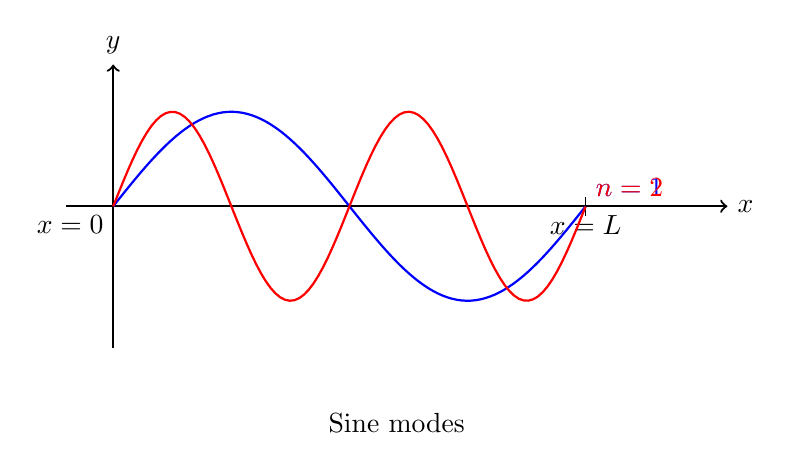
\begin{tikzpicture}[scale=1.2]
    % Sine waves
    \draw[thick, ->] (-0.5, 0) -- (6.5, 0) node[right] {$x$};
    \draw[thick, ->] (0, -1.5) -- (0, 1.5) node[above] {$y$};
    \node[below left] at (0,0) {$x=0$};
    \node[below] at (5,0) {$x=L$};
    \draw (5, 0.1) -- (5, -0.1);
    
    \draw[thick, blue, domain=0:5, samples=100] plot (\x, {sin(\x*360/5)}) node[above right] {$n=1$};
    \draw[thick, red, domain=0:5, samples=100] plot (\x, {sin(\x*720/5)}) node[above right] {$n=2$};
    \node[above] at (3, -2.5) {Sine modes};
\end{tikzpicture}
\quad
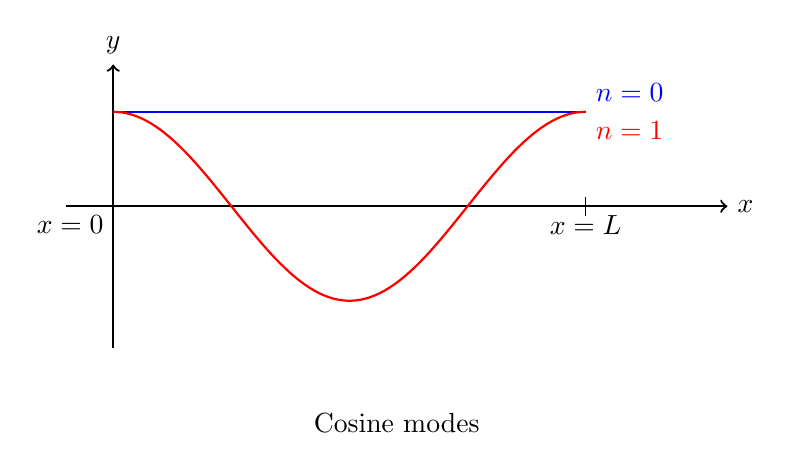
\begin{tikzpicture}[scale=1.2]
    % Cosine waves
    \draw[thick, ->] (-0.5, 0) -- (6.5, 0) node[right] {$x$};
    \draw[thick, ->] (0, -1.5) -- (0, 1.5) node[above] {$y$};
    \node[below left] at (0,0) {$x=0$};
    \node[below] at (5,0) {$x=L$};
    \draw (5, 0.1) -- (5, -0.1);
    
    \draw[thick, blue, domain=0:5] plot (\x, {1}) node[above right] {$n=0$};
    \draw[thick, red, domain=0:5, samples=100] plot (\x, {cos(\x*360/5)}) node[below right] {$n=1$};
    \node[above] at (3, -2.5) {Cosine modes};
\end{tikzpicture}
\end{center}

\textbf{Orthogonality relations:}
If we denote $\langle f, g \rangle := \int_0^L f(x)g(x) \dd x$ (this is indeed an "inner-product" on the space of functions on $[0,L]$):
$$\left\langle \sin\left(\frac{2\pi n}{L} x\right), \sin\left(\frac{2\pi m}{L} x\right) \right\rangle = \begin{cases} \frac{L}{2}, & n = m \ne 0 \\ 0, & n \ne m \end{cases}$$
Same for cosines: $\langle \cos(\frac{2\pi n}{L}x), \cos(\frac{2\pi m}{L}x) \rangle$.
Also, $\langle \sin(\frac{2\pi n}{L}x), \cos(\frac{2\pi m}{L}x) \rangle = 0$ for all $n,m$.
We use these functions as an orthogonal basis to decompose other functions.

\textbf{Trigonometric (Fourier) series:}
Given a function $f: [0,L] \rightarrow \R$ which is piecewise continuous, can we decompose:
$$f(x) = \frac{a_0}{2} + \sum_{n=1}^{\infty} \left( a_n \cdot \cos\left(\frac{2\pi n}{L}x\right) + b_n \cdot \sin\left(\frac{2\pi n}{L}x\right) \right) ?$$
(The same considerations hold in the case when $f: \R \rightarrow \R$ is periodic with period $L$; I can think of it as a function on $[0,L]$).

The answer is yes! Note that if such a decomposition exists, I can compute (formally) the coefficients because of the orthogonality conditions:
\begin{align*}
\int_0^L f(x) \dd x &= \frac{L}{2} a_0 \\
\int_0^L f(x) \cos\left(\frac{2\pi n}{L} x\right) \dd x &= \frac{L}{2} a_n, \quad n=1,2,\dots \\
\int_0^L f(x) \sin\left(\frac{2\pi n}{L} x\right) \dd x &= \frac{L}{2} b_n, \quad n=1,2,\dots
\end{align*}

So it makes sense to define:
\begin{align*}
a_n &= \frac{2}{L} \int_0^L f(x) \cdot \cos\left(\frac{2\pi n}{L} x\right) \dd x, \quad n=0,1,2,\dots \\
b_n &= \frac{2}{L} \int_0^L f(x) \cdot \sin\left(\frac{2\pi n}{L} x\right) \dd x, \quad n=1,2,\dots
\end{align*}

\begin{theorem}[Dirichlet's Theorem]
Assume that $f: [0,L] \rightarrow \R$ is piecewise continuous. Let $f_N(x)$ denote the partial sum:
$$f_N(x) = \frac{a_0}{2} + \sum_{n=1}^N \left( a_n \cos\left(\frac{2\pi n}{L} x\right) + b_n \sin\left(\frac{2\pi n}{L} x\right) \right)$$
Then $\lim_{N\rightarrow+\infty} f_N(x) = f(x)$ at every point $x$ where $f$ is differentiable. Moreover:
$$\int_0^L |f_N(x) - f(x)| \dd x \xrightarrow{N\rightarrow+\infty} 0$$
At points of jump discontinuities, $f_N(x)$ converges to the midpoint:
$$f_N(x) \longrightarrow \frac{f(x^+) + f(x^-)}{2}$$
\end{theorem}

\begin{center}
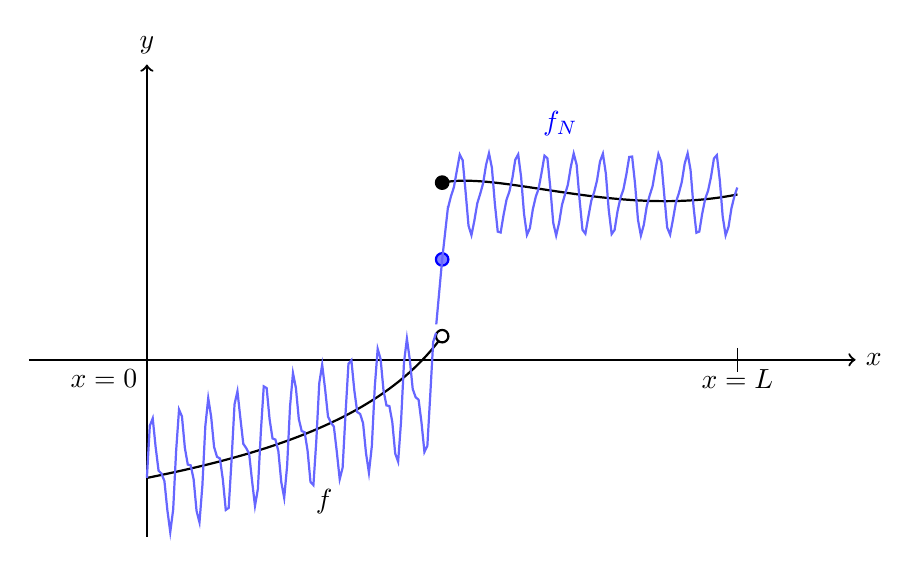
\begin{tikzpicture}[scale=1.5]
    % Axes
    \draw[thick, ->] (-1, 0) -- (6, 0) node[right] {$x$};
    \draw[thick, ->] (0, -1.5) -- (0, 2.5) node[above] {$y$};
    \node[below left] at (0,0) {$x=0$};
    \node[below] at (5,0) {$x=L$};
    \draw (5, 0.1) -- (5, -0.1);
    
    % Function with jump
    \draw[thick, black] (0, -1) .. controls (1, -0.8) and (2, -0.5) .. (2.5, 0.2);
    \draw[thick, black] (2.5, 1.5) .. controls (3, 1.6) and (4, 1.2) .. (5, 1.4);
    
    % Jump markers
    \filldraw[fill=white, draw=black, thick] (2.5, 0.2) circle (1.5pt);
    \filldraw[fill=black, draw=black, thick] (2.5, 1.5) circle (1.5pt);
    \filldraw[fill=blue!50!white, draw=blue, thick] (2.5, 0.85) circle (1.5pt); % Midpoint
    
    % Approximating Fourier sum (wavy)
    \draw[thick, blue!60!white, domain=0:2.45, samples=100] plot (\x, {-1 + 0.3*\x + 0.4*sin(1500*\x) + 0.2*sin(3000*\x)});
    \draw[thick, blue!60!white, domain=2.55:5, samples=100] plot (\x, {1.4 + 0.3*cos(1500*\x) + 0.1*sin(3000*\x)});
    \draw[thick, blue!60!white] (2.45, 0.3) -- (2.5, 0.85) -- (2.55, 1.3);
    
    \node[black] at (1.5, -1.2) {$f$};
    \node[blue] at (3.5, 2.0) {$f_N$};
\end{tikzpicture}
\end{center}

\textbf{Special cases:}
\begin{itemize}
    \item \textbf{When $f$ is odd} ($f(-x) = -f(x)$): Then $a_n = 0$ for all $n$, and
    $$f(x) = \sum_{n=1}^\infty b_n \cdot \sin\left(\frac{2\pi n}{L} x\right)$$
    with $b_n = \frac{2}{L} \int_0^L f(x) \cdot \sin\left(\frac{2\pi n}{L} x\right) \dd x = \frac{4}{L} \int_0^{L/2} f(x) \sin\left(\frac{2\pi n}{L} x\right) \dd x$.
    (Here, use the fact that the integral over any interval of length $L$ is the same since the product is $L$-periodic).
    
    \item \textbf{When $f$ is even} ($f(-x) = f(x)$): Then $b_n = 0$ for all $n$, and
    $$f(x) = \frac{a_0}{2} + \sum_{n=1}^\infty a_n \cdot \cos\left(\frac{2\pi n}{L} x\right)$$
    with $a_n = \frac{4}{L} \int_0^{L/2} f(x) \cos\left(\frac{2\pi n}{L} x\right) \dd x$.
\end{itemize}

The functions $e_n(x) = \cos(\frac{2\pi n}{L}x)$ and $h_n(x) = \sin(\frac{2\pi n}{L}x)$ are sometimes called modes. Note that $e_n'(0) = 0 = e_n'(L)$ and $h_n(0) = 0 = h_n(L)$.

\newpage

\subsubsection{Solving the 1-Dimensional Heat Equation}

Let's return to the 1-dimensional heat equation:
\begin{equation}
\begin{cases}
\frac{\partial u}{\partial t} - \frac{\partial^2 u}{\partial x^2} = f & \text{for } t > 0, 0 < x < L \\
u|_{t=0} = u_0 & \text{(initial condition)} \\
u|_{x=0} = 0, \quad u|_{x=L} = 0 & \text{(boundary conditions)}
\end{cases}
\end{equation}

\textbf{Overview of the method:}
\begin{enumerate}
    \item Decompose the heat equation into Fourier modes (in $x$).
    \item The PDE becomes an ODE (in time) for the Fourier coefficients: Solve it.
    \item Find a formula for the solution by summing the mode solutions.
\end{enumerate}

\begin{theorem}[Uniqueness]
The initial-boundary value problem for the heat equation has a unique solution.
\end{theorem}
\begin{proofbox}
If $u_1, u_2$ are two solutions, then $v = u_1 - u_2$ solves the homogeneous problem:
$\frac{\partial v}{\partial t} - \frac{\partial^2 v}{\partial x^2} = 0$, $v|_{t=0} = 0$, $v|_{x=0} = v|_{x=L} = 0$.
Then using the energy method:
\begin{align*}
\frac{\dd}{\dd t} \left( \int_0^L v^2(x,t) \dd x \right) &= \int_0^L 2 v \frac{\partial v}{\partial t} \dd x = 2 \int_0^L v \frac{\partial^2 v}{\partial x^2} \dd x \\
&= 2 \left[ v \cdot \frac{\partial v}{\partial x} \right]_{x=0}^{x=L} - 2 \int_0^L \left(\frac{\partial v}{\partial x}\right)^2 \dd x \\
&= -2 \int_0^L \left(\frac{\partial v}{\partial x}\right)^2 \dd x \le 0
\end{align*}
So $\int_0^L v^2(x,t) \dd x$ is decreasing. Since $v(x,0) = 0$, we have $\int_0^L v^2(x,t) \dd x \le \int_0^L v^2(x,0) \dd x = 0$.
Thus $v(x,t) = 0$ for all $t \ge 0, 0 \le x \le L$.
\end{proofbox}

So, in view of uniqueness, if we can find a solution in any way, then that is the unique solution.

\textbf{Fourier Decomposition Trick:}
To decompose into Fourier modes, it helps to do the following trick (since we want $u|_{x=0} = 0, u|_{x=L} = 0$): Extend $u(t,x)$ in $x$ to a $2L$-periodic function on $\R$ which is odd. Do the same for $u_0, f$.

Note: If $u$ is a $2L$-periodic and odd function which is continuous, then necessarily $u|_{x=0} = 0$ and $u|_{x=L} = 0$.

Fourier series (with respect to the period $2L$):
$$u(x,t) = \sum_{n=1}^\infty b_n(t) \cdot \sin\left(\frac{2\pi n}{2L} x\right) = \sum_{n=1}^\infty b_n(t) \cdot \sin\left(\frac{\pi n}{L} x\right)$$
where $b_n(t) = \frac{2}{L} \int_0^L u(x,t) \cdot \sin\left(\frac{\pi n}{L} x\right) \dd x$.

Similarly, decompose the known data:
$$u_0(x) = \sum_{n=1}^\infty b_{0n} \cdot \sin\left(\frac{\pi n}{L} x\right), \quad f(x,t) = \sum_{n=1}^\infty f_n(t) \cdot \sin\left(\frac{\pi n}{L} x\right)$$

Differentiating the series formally:
\begin{align*}
\frac{\partial u}{\partial x}(x,t) &= \sum_{n=1}^\infty b_n(t) \cdot \frac{\pi n}{L} \cdot \cos\left(\frac{\pi n}{L} x\right) \\
\frac{\partial^2 u}{\partial x^2}(x,t) &= \sum_{n=1}^\infty b_n(t) \cdot \left(-\frac{\pi^2 n^2}{L^2}\right) \cdot \sin\left(\frac{\pi n}{L} x\right) \\
\frac{\partial u}{\partial t}(x,t) &= \sum_{n=1}^\infty b_n'(t) \cdot \sin\left(\frac{\pi n}{L} x\right)
\end{align*}

Injecting into the PDE $\frac{\partial u}{\partial t} - \frac{\partial^2 u}{\partial x^2} = f$ gives:
$$\sum_{n=1}^\infty \left( b_n'(t) + \frac{\pi^2 n^2}{L^2} b_n(t) \right) \cdot \sin\left(\frac{\pi n}{L} x\right) = \sum_{n=1}^\infty f_n(t) \cdot \sin\left(\frac{\pi n}{L} x\right)$$

\begin{verification}[Correction of the ODE sign]
In the raw notes, the equation was written as $b_n' - \frac{\pi^2 n^2}{L^2} b_n = f_n$. However, taking $\frac{\partial u}{\partial t} - \frac{\partial^2 u}{\partial x^2}$, the double spatial derivative already introduces a negative sign ($-\frac{\pi^2 n^2}{L^2}$). Subtracting it yields a positive term: $b_n' - (-\dots) = b_n' + \frac{\pi^2 n^2}{L^2} b_n$. This yields the correct stable decay expected for the heat equation.
\end{verification}

So, by equating coefficients, we obtain a family of ODEs:
$$b_n'(t) + \frac{\pi^2 n^2}{L^2} b_n(t) = f_n(t) \quad \text{for } n=1,2,3,\dots \text{ and } t > 0$$

The initial conditions $u(x,0) = u_0(x)$ imply $b_n(0) = b_{0n}$.
The above is an initial value problem of the standard form $y' + ay = g(t)$, $y(0) = y_0$, which we can solve using the integrating factor method or the Laplace transform.

\textbf{Solution:}
$$b_n(t) = b_{0n} \cdot e^{-\frac{\pi^2 n^2}{L^2} t} + \int_0^t e^{-\frac{\pi^2 n^2}{L^2} (t-s)} f_n(s) \dd s$$

So we have found $u$:
$$u(x,t) = \sum_{n=1}^\infty b_n(t) \sin\left(\frac{\pi n}{L} x\right)$$

\textbf{Remarks:}
\begin{itemize}
    \item \textbf{If $f=0$:} $u(x,t) = \sum_{n=1}^\infty b_{0n} e^{-\frac{\pi^2 n^2}{L^2} t} \cdot \sin\left(\frac{\pi n}{L} x\right)$. 
    The solution decays exponentially fast to 0 as $t \rightarrow +\infty$ (and faster decay occurs in higher modes).
    
    \item \textbf{Special solutions:} If $u_0 = 0$ and $f(x,t) = \sin(\frac{\pi x}{L})$:
    Then $f_n(t) = 1$ for $n=1$ and $0$ for $n \ge 2$.
    $\implies b_1(t) = \int_0^t e^{-\frac{\pi^2}{L^2}(t-s)} \cdot 1 \dd s = \frac{L^2}{\pi^2} \left(1 - e^{-\frac{\pi^2}{L^2} t}\right)$ and $b_n(t) = 0$ for $n \ge 2$.
    $$u(x,t) = \frac{L^2}{\pi^2} \left(1 - e^{-\frac{\pi^2}{L^2} t}\right) \cdot \sin\left(\frac{\pi x}{L}\right)$$
    
    \item \textbf{Neumann Boundary Conditions:}
    If we wanted Neumann boundary conditions (namely $\frac{\partial u}{\partial x}\big|_{x=0} = 0 = \frac{\partial u}{\partial x}\big|_{x=L}$), we would extend $u$ as an \textit{even} $2L$-periodic function. In that case:
    $$u(x,t) = \frac{a_0(t)}{2} + \sum_{n=1}^\infty a_n(t) \cdot \cos\left(\frac{\pi n x}{L}\right)$$
\end{itemize}